% \pagebreak[4]
% \hspace*{1cm}
% \pagebreak[4]
% \hspace*{1cm}
% \pagebreak[4]
%\usepackage[round,colon,authoryear]{natbib}

\chapter{A pipeline for the analysis of TraDIS experiments, with an application to {\it Salmonella} macrophage invasion}
\label{sec:chapterPingpong}
\ifpdf
    \graphicspath{{Chapter3/Chapter3Figs/EPS/}{Chapter3/Chapter3Figs/}}
\fi

\textit{Section 3.2 describes a collaborative study with Gemma C. Langridge (Pathogen Genomics, Wellcome Trust Sanger Institute). Gemma performed all laboratory experiments described in this chapter.}

\section{Introduction}

In the previous chapter, I described the results of a study predicting and comparing the genes required for robust growth of two \textit{Salmonella} serovars in standard laboratory media. While this revealed interesting aspects of \textit{Salmonella} biology, linking these findings to \textit{Salmonella}'s infective niche in the human host is difficult. However, transposon-insertion sequencing can be used to interrogate infective conditions directly (reviewed previously in section 1.5): by comparing libraries passed through a condition of interest to control libraries, we can determine the genomic regions involved in survival in that condition. In this chapter, I describe a pipeline for the analysis of such experiments, illustrated with an experiment assaying genes required for \textit{S.} Typhi and Typhimurium invasion of (or uptake into) human macrophage.

\subsection{\textit{Salmonella} interactions with macrophage}

As previously described in section 2.1, the ability to invade and survive in host cells was a major factor in the early evolution of \textit{S. enterica} subspecies \textit{enterica}; survival in macrophages in particular is known to be necessary for virulence \parencite{Fields1986}. This ability appears to have been largely driven by the acquisition of two horizontally-acquired pathogenicity islands, SPI-1 and -2. Due to the availability of a mouse model of systemic infection \parencite{Santos2001}, most of what is known about \textit{Salmonella} interactions with host cells is derived from studies of \textit{S.} Typhimurium infection.

\textit{S.} Typhimurium infections of either epithelial or phagocytic cells appear to follow broadly similar paths (\textcite{Figueira2012}, see also figure \ref{fig:SCV}). On encountering a suitable host cell, the bacterium adheres using an array of fimbrial adhesins \parencite{Baumler1996a, Velden1998}. The SPI-1 T3SS, a needle-like complex spanning the periplasm and presenting its tip to the exterior of the bacterial cell \parencite{Mueller2008}, induces membrane ruffling in the host cell through secretion of effector proteins \parencite{Zhou2001}, facilitating bacterial uptake. While use of this mechanisms is not strictly necessary for entrance to phagocytic cells such as macrophage, {\it S.} Typhimurium strains unable to induce ruffling are taken up six to ten times less efficiently than the wild-type \parencite{Monack1996}, though the entry mechanism does not ultimately affect cell fate \parencite{Rathman1997}.

Once entry has been gained to the cell, through either active invasion or phagocytic engulfment, {\it S.} Typhimurium begins expressing a second T3SS encoded by SPI-2. The effectors secreted by this T3SS allow {\it S.} Typhimurium to remodel the \textit{Salmonella} containing vacuole (SCV)\nomenclature[Z]{SCV}{\textit{Salmonella} containing vacuole}, and even modulate host immune signalling (see figure \ref{fig:SCV}). There is some controversy as to whether or not the SCV undergoes fusion with lysosomes; a recent study suggests it does, but that the activity of these lysosomes is first modulated by the SPI-2 effector SifA \parencite{McGourty2012}. Little is known about the growth conditions {\it S.} Typhimurium faces within the SCV, though transcriptomic studies suggests it is aerobic, mildly acidic, rich in gluconate, and limited in aromatic amino acids, purines, and pyrimidines \parencite{Eriksson2003, Hautefort2008}.

Our understanding of how these findings relate to {\it S.} Typhi infections of human macrophage is limited, largely due to the lack of a non-human model organism for this serovar. A recent study suggests that SPI-2 may not even be necessary for {\it S.} Typhi invasion of and survival in human macrophages \parencite{Forest2010}, though SPI-2 genes are known to be expressed by {\it S.} Typhi in macrophages \parencite{Faucher2006} and a SPI-2 deletion mutant was previously shown to be attenuated under these conditions \parencite{Khan2003}. Regardless, it is well established that the genotype of both the \textit{Salmonella} strain used and the macrophage can have profound effects on the course of infection. A number of studies comparing a variety of \textit{Salmonella} serovars infecting murine-, human-, and even chicken-derived macrophages have repeatedly shown that serovars exhibit remarkably different behaviors under the same conditions \parencite{Vladoianu1990, Schwan2000, Okamura2005}; these differences appear to correlate somewhat with the degree of host-adapation exhibited by the serovar. In this study we compare our \textit{Salmonella} TraDIS libraries following uptake by human macrophage in the hopes of uncovering genomic factors underlying these differences in behavior.

\begin{figure}[htp]
\begin{center}
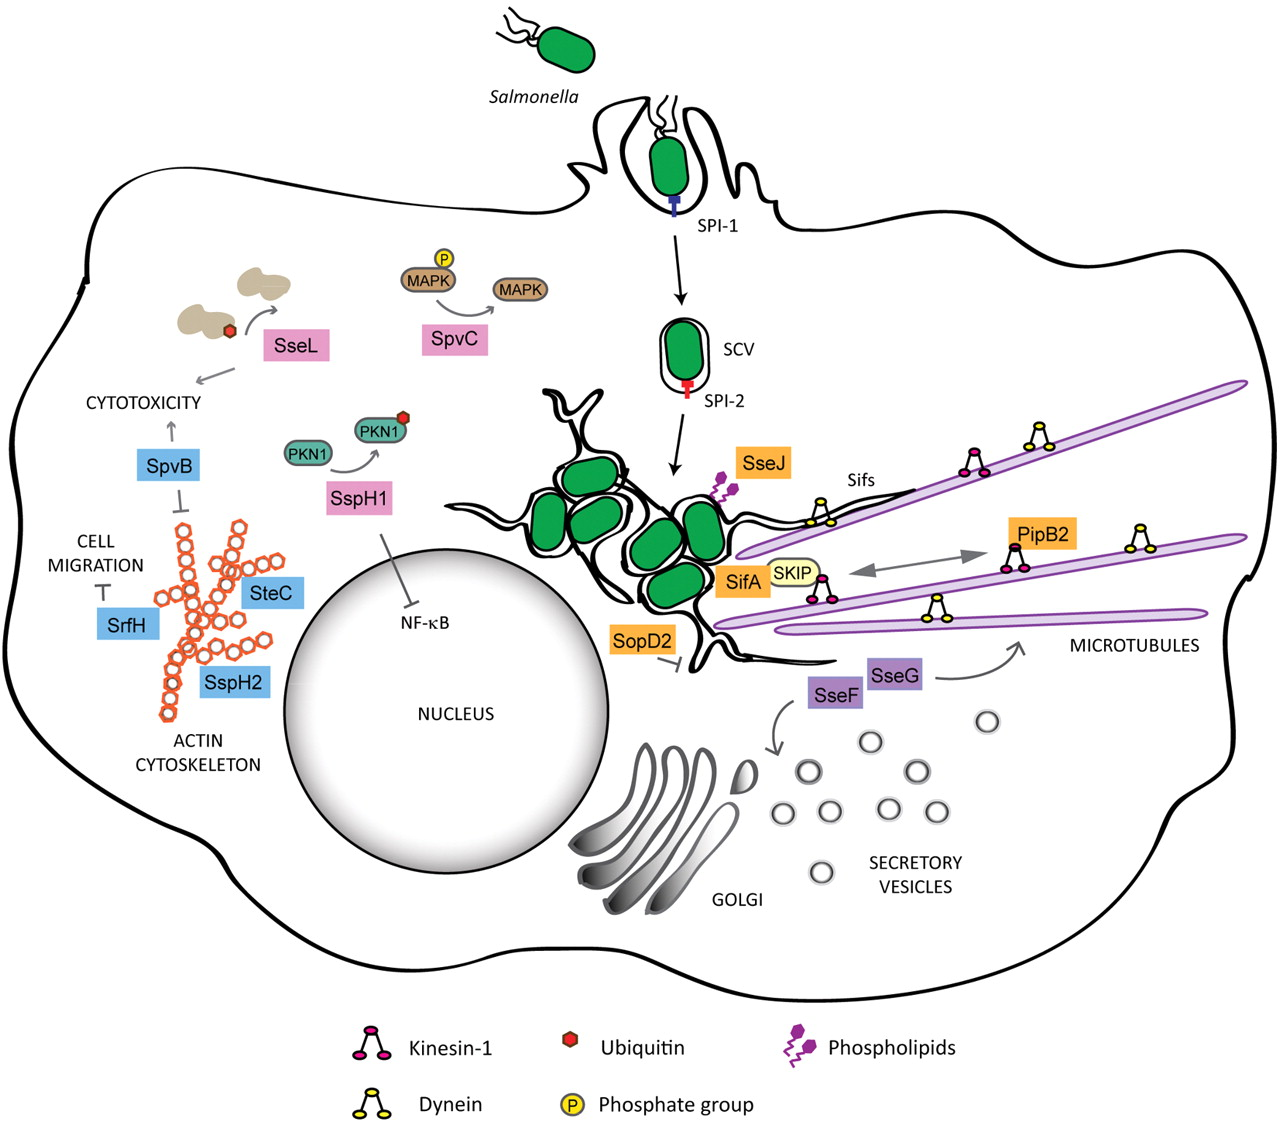
\includegraphics[width=14cm]{SCV.jpg}
\caption[Biogenesis of the \textit{Samonella} containing vacuole]{\textbf{Biogenesis of the \textit{Samonella} containing vacuole (SCV).} \textit{Salmonella} adheres to the outer membrane of host cells, and uses the SPI-1 T3SS and its associated effectors to induce membrane ruffling and entry into the SCV. The SPI-2 T3SS functions mainly in maintenance of the SCV, through the action of the effectors SifA, SopD2, SseJ and PipB2 (orange boxes), and its localization near the Golgi of host cells, mediated by SseF and SseG (purple boxes). Other effectors are involved in modulation of host immune signalling (SpvC, SspH1 and SseL; pink boxes) or target the host cytoskeleton (SteC, SpvB, SspH2 and SrfH; blue boxes). Reproduced from \textcite{Figueira2012} under a Creative Commons Attribution License (CCAL). 
} 
\label{fig:SCV}
\end{center}
\end{figure}

\subsection{Conditional gene fitness}

Determining conditional gene fitness presents a somewhat different problem to that addressed in the previous chapter, predicting and comparing ``essential'' genes under the conditions of library creation. In predicting gene essentiality, we had a single time point representing the initial growth of the library on rich media, while in identifying conditional gene fitness (measured as the relative expansion or contraction of mutant populations) we are always comparing changes in mutant fitness with respect to fitness in a baseline condition. The ratio of reads between the two conditions is taken as indicative of relative mutant prevalences between them. In some ways, this makes the problem of identifying genes with strong fitness effects easier: as we are primarily interested in the ratio of various insertion mutants present between the two conditions, effects that may confound the prediction of simple gene essentiality are effectively ``zeroed out''. More explicitly, whether low insertion density in the initial library occurs due to chance, nucleotide composition bias, or the exclusionary effects of high-density DNA-binding proteins (described in section 2.3.3) does not matter -- these regions can simply be identified as not producing sufficient reads over insertion-sites to be assayed and removed from the analysis.

In many ways, the problem of investigating the statistical and biological significance of ratios of reads over insertion sites resembles established analyses developed for differential RNA-seq analysis. In the following sections I describe the application of these methods to the problem of determining conditional gene fitness.

\section{Methods}
\textit{Gemma C. Langridge performed all laboratory experiments described in this chapter. A more detailed description of the experimental methods is available in \textcite{Langridge2010}, including preliminary assessments of bacterial strain ability to grow in RPMI\nomenclature[Z]{RPMI}{Rosewell Park Memorial Institute (cell culture medium)}, invade THP-1 derived macrophage, and experiment optimization.}

\subsection{Strains and cell lines}
These experiments were performed with \textit{S.} Typhi WT174 and  \textit{S.} Typhimurium SL3261 transposon mutant libraries, described in Chapter 3. Human monocytic cell line THP-1 was used for cell infections.

\subsection{Preparation of THP-1 cells}

\subsection{Mapping insertion sites}

\subsection{Defining genomic features}

\subsection{Quality control}

\subsection{Inter-library normalization}

\subsection{Identifying fitness effects}

\subsection{Functional analysis of gene sets that affect fitness}

\section{Application: \textit{Salmonella enterica} macrophage invasion}

\subsection{Background: the {\it Salmonella} containing vacuole}

\subsection{Experimental methods}

\textit{All experiments were performed by Gemma Langridge. They are described here briefly for completeness; in-depth descriptions of the experiments are available in \parencite{Langridge2010}}


\subsection{Results}

\subsection{Other applications}